\chapter{The Residue Theorem \& Applications} % Main chapter title

\begin{theorem}
    [Residue Theorem]
    Suppoes $f$ is analytic on a simply connected domain $D$, except for a finite number of isolated singularities at $z_1, z_2, \cdots, z_n \in D$. Let $\gamma$ be a piecewise $C^1$, positively oriented, simple closed curve in $D$ which does not pass through any of the singularities. Then:
    \begin{equation}
        \boxed{\oint_{\gamma} f(z) dz = 2\pi i \sum_{z_k \text{ inside } \gamma} \text{Res}(f, z_k)}
    \end{equation}
\end{theorem}
\begin{figure}[H]
    \centering
    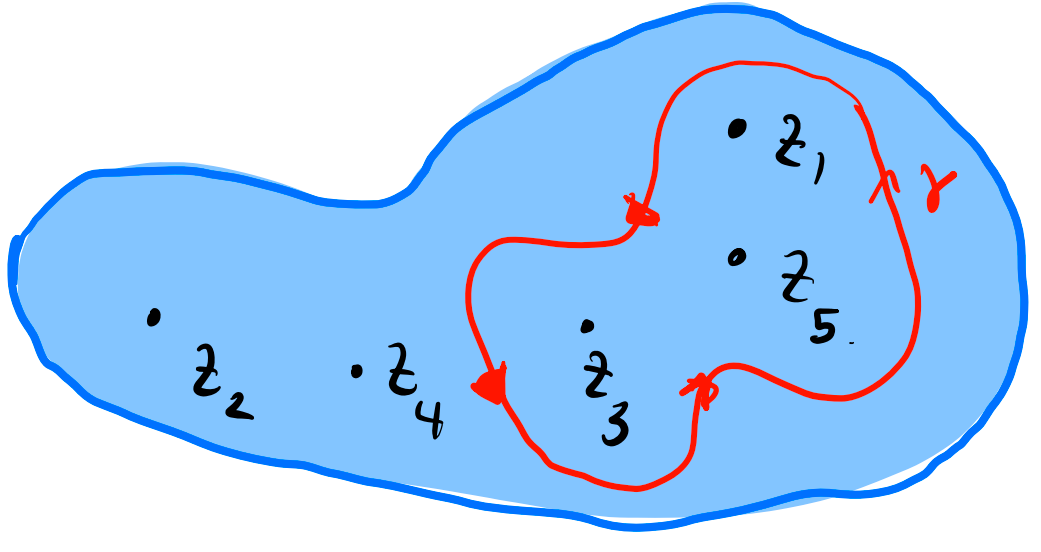
\includegraphics[width=0.4\textwidth]{LECTURE_11/residues.png}
    \caption{Residue Theorem}
    \label{fig:residue}
\end{figure}

\begin{proof}
    Let $\gamma_1, \gamma_2, \cdots, \gamma_n$ be disjoin, positively oriented, circles around $z_1, z_2, \cdots, z_n$ respectively. We apply Green's theorem to get:
    \begin{equation*}
        \oint_{\gamma} f(z) dz = \sum_{k : z_k \text{ inside } \gamma} \oint_{\gamma_k} f(z) dz
    \end{equation*}
    \begin{figure}[H]
        \centering
        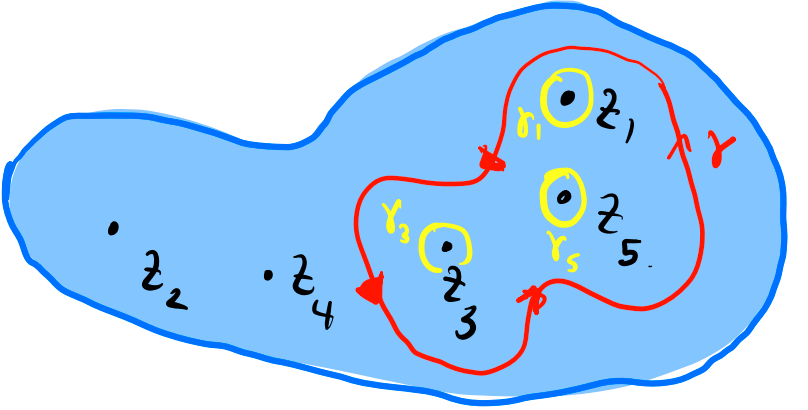
\includegraphics[width=0.4\textwidth]{LECTURE_11/residues-2.png}
        \caption{circles around $z_1, z_2, \cdots, z_n$}
        \label{fig:residue-2}
    \end{figure}

    But now by the Cauchy Integral Formula

    \begin{equation*}
        \oint_{\gamma_k} f(z) dz = 2\pi i \text{Res}(f, z_k)
    \end{equation*}

\end{proof}

\begin{example}
    Compute:
    \begin{equation*}
        \int_{-\infty}^{\infty} \frac{x}{((1 + x^2)(4+ x^2))} dx
    \end{equation*}

    \textbf{Step 1:} Change to a complex integral:
    \begin{equation*}
        P(z) = z^2, \quad Q(z) = (1 + z^2)(4 + z^2)
    \end{equation*}

    \textbf{Step 2:} Choose a contour:
    \begin{figure}[H]
        \centering
        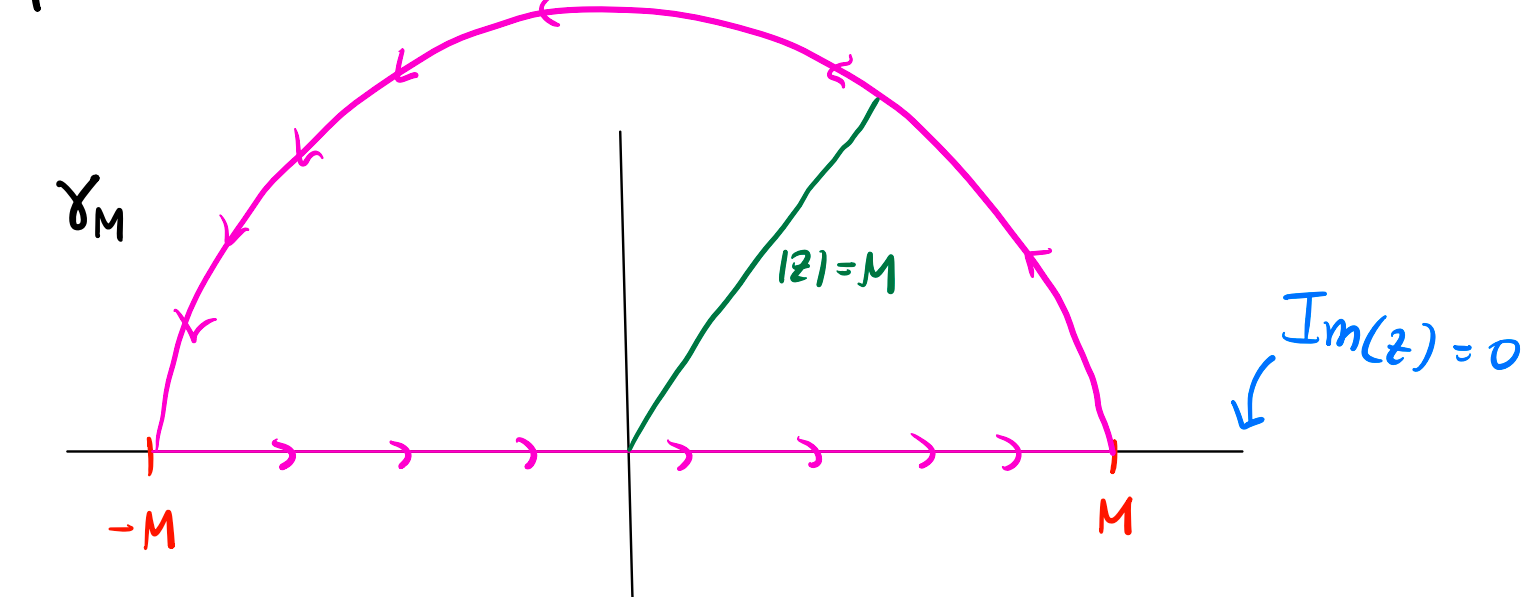
\includegraphics[width=0.4\textwidth]{LECTURE_11/contour.png}
        \caption{Contour}
        \label{fig:contour}
    \end{figure}
    Suppose $M$ is very large
    \begin{enumerate}
        \item $\int_{\gamma_M} \frac{P(z)}{Q(z)} dz$ can be computed by the residue formula.
        \item On the other hand:
              \begin{equation*}
                  \int_{\gamma_M} \frac{P(z)}{Q(z)} dz = \underbrace{\int_{-M}{M}\frac{x^2}{(1 + x^2)(4 + x^2)} dx}_{\text{The integral we want}} + \int_{0}{\pi} \frac{P(M e^{i\theta})}{Q(M e^{i\theta})} i M e^{i\theta} d\theta
              \end{equation*}
    \end{enumerate}
    \underline{Now}:
    \begin{align*}
        |P(Me^{i\theta})| & \leq M^2                                                \\
        |Q(Me^{i\theta})| & = |(Me^{i\theta})^2 + 1||(Me^{i\theta})^2 + 4|
                          & \geq \frac{1}{10} M^4 \qquad \text{for a very large } M
    \end{align*}
    \underline{So}
    \begin{equation*}
        \left| \int_0^\pi \frac{P(Me^{i\theta})}{Q(Me^{i\theta})} i M e^{i\theta} d\theta \right| \leq 10 \pi \frac{M^3}{M^4} \to 0 \quad \text{as } M \to \infty
    \end{equation*}
    \textbf{\underline{Thus}}
    \begin{equation*}
        \int_{-\infty}^{\infty} \frac{x^2}{(1 + x^2)(4 + x^2)} dx = \lim_{M \to \infty} \int_{\gamma_M} \frac{P(z)}{Q(z)} dz
    \end{equation*}
    Which can be computed using the residue formula. \\
    $Q(z)$ has zeroes at $z = \pm i, \pm 2i$. only $+i, +2i$ are inside $\gamma_M$ for large $M$. So:
    \begin{align*}
        \rightarrow \boxed{z = i} \quad \frac{z^2}{(z + i)(z-i)(z^2 + 4)}  & = \frac{1}{z - i}\left[\frac{z^2}{(z + i)(z^2 + 4)}\right] \\
        \text{Res}(f, i)                                                   & = \frac{i^2}{(i + i)(i^2 + 4)} = \frac{-1}{6i}             \\
        \rightarrow \boxed{z = 2i} \quad \frac{z^2}{(z + i)(z-i)(z^2 + 4)} & = \frac{1}{z - 2i}\left[\frac{z^2}{(z + i)(z - i)}\right]
    \end{align*}
    end
\end{example}